% ---
% Capa
% ---
\imprimircapa
% ---

% ---
% Folha de rosto
% (o * indica que haverá a ficha bibliográfica)
% ---
\imprimirfolhaderosto
% ---

% ---
% Inserir a ficha bibliografica
% ---
% % http://ficha.bu.ufsc.br/
% \begin{fichacatalografica}
% 	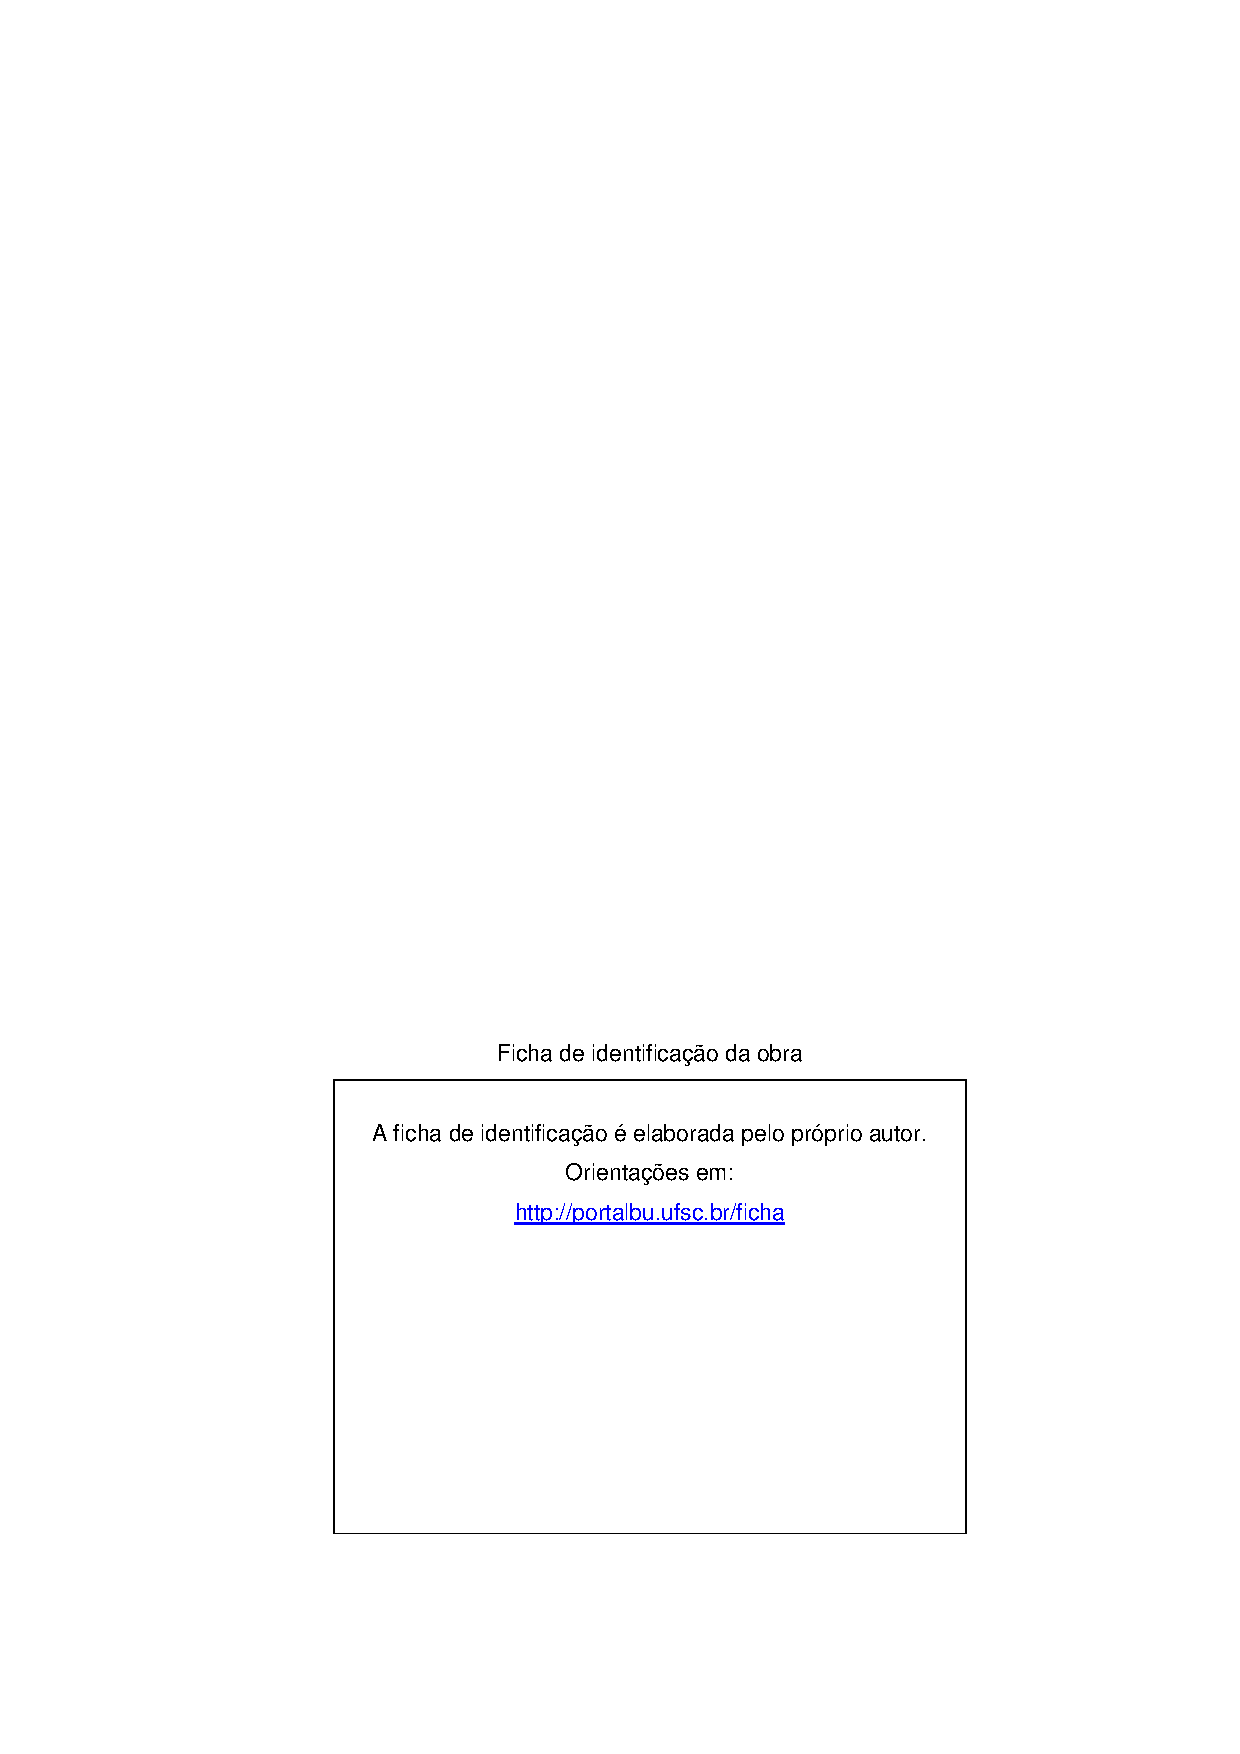
\includepdf{beforetext/Ficha_Catalografica.pdf}
% \end{fichacatalografica}
% ---

% ---
% Inserir folha de aprovação
% ---
\begin{folhadeaprovacao}
	\OnehalfSpacing
	\centering
	\imprimirautor\\%
	\vspace*{10pt}		
	\textbf{\imprimirtitulo}%
	\ifnotempty{\imprimirsubtitulo}{:~\imprimirsubtitulo}\\%
	%		\vspace*{31.5pt}%3\baselineskip
	\vspace*{\baselineskip}
    
	%\begin{minipage}{\textwidth}
	% ~do~\imprimirprograma~do~\imprimircentro~da~\imprimirinstituicao~para~a~obtenção~do~título~de~\imprimirformacao.
	Este~\imprimirtipotrabalho~foi julgado adequado para obtenção do Título de “\imprimirformacao” e aprovado em sua forma final pelo~\imprimirprograma~do~\imprimirinstituicao~--~Campus São Borja. \\
		\vspace*{\baselineskip}
	\imprimirlocal, \imprimirdata. \\
	\vspace*{2\baselineskip}
	% \assinatura{\OnehalfSpacing\imprimircoordenador \\ \imprimircoordenadorRotulo~do Curso}
	\vspace*{2\baselineskip}
	\textbf{Banca Examinadora:} \\
	\vspace*{\baselineskip}
	\assinatura{\OnehalfSpacing\imprimirorientador \\ \imprimirorientadorRotulo}
	%\end{minipage}%
	\vspace*{\baselineskip}
	\assinatura{Prof.(a) xxxx, Dr(a).\\
	Avaliador(a) \\
	Instituição xxxx}

	\vspace*{\baselineskip}
	\assinatura{Prof.(a) xxxx, Dr(a).\\
	Avaliador(a) \\
	Instituição xxxx}


\end{folhadeaprovacao}
% ---

% ---
% Dedicatória
% ---
\begin{dedicatoria}
	\vspace*{\fill}
	\noindent
	% \begin{adjustwidth*}{}{5.5cm}     
    \begin{flushright}
		Este trabalho é dedicado aos meus colegas de \\classe e aos meus queridos pais.
	\end{flushright}
\end{dedicatoria}
% ---

% ---
% Agradecimentos
% ---
\begin{agradecimentos}
	Inserir os agradecimentos aos colaboradores à execução do trabalho. 
	
	Xxxxxxxxxxxxxxxxxxxxxxxxxxxxxxxxxxxxxxxxxxxxxxxxxxxxxxxxxxxxxxxxxxxxxx. 
\end{agradecimentos}
% ---

% ---
% Epígrafe
% ---
\begin{epigrafe}
	\vspace*{\fill}
	\begin{flushright}
		\textit{``Texto da Epígrafe.\\
			Citação relativa ao tema do trabalho.\\
			É opcional. A epígrafe pode também aparecer\\
			na abertura de cada seção ou capítulo.\\
			Deve ser elaborada de acordo com a NBR 10520.''\\
			(Autor da epígrafe, ano)}
	\end{flushright}
\end{epigrafe}
% ---

% ---
% RESUMOS
% ---

% resumo em português
\setlength{\absparsep}{18pt} % ajusta o espaçamento dos parágrafos do resumo
\begin{resumo}
	\SingleSpacing
	O Diabetes Mellitus tipo 2 apresenta elevada proporção de casos não diagnosticados no Brasil, e a triagem na Atenção Primária à Saúde demanda estratégias capazes de priorizar quem encaminhar a exame laboratorial. Diante disso, o presente trabalho teve como objetivo desenvolver um modelo classificatório de aprendizado de máquina para identificar indivíduos com perfil associado à hiperglicemia crônica, definida por hemoglobina glicada igual ou superior a 6,5\%, a partir de variáveis não invasivas da Subamostra Laboratorial da Pesquisa Nacional de Saúde de 2013. A pesquisa, de natureza aplicada e abordagem quantitativa, seguiu a metodologia CRISP-DM sobre uma amostra analítica de 8.451 adultos, dividida em conjuntos de treino e de teste. Foram comparados a Regressão Logística e o \textit{Random Forest}, com aprendizagem sensível ao custo para o tratamento do desbalanceamento das classes, limiar de decisão calibrado para a sensibilidade de 0,80 e explicabilidade por meio do método SHAP. No conjunto de teste, os modelos alcançaram AUC-ROC entre 0,770 e 0,786, e o modelo de referência, o \textit{Random Forest}, obteve sensibilidade de 0,807, encaminhando a exame 40,5\% dos indivíduos, contra 84,0\% de uma regra clínica baseada na idade e no índice de massa corporal. No regime de sensibilidade equiparada à da regra, entretanto, o modelo de referência não cumpriu o critério de sucesso estabelecido, e as probabilidades produzidas mostraram-se descalibradas, de maneira que as saídas foram tratadas como escores de ordenação, e não como estimativas de risco individual. A explicabilidade indicou a idade e a circunferência da cintura como as variáveis de maior contribuição, ordenação que se manteve estável entre dois regimes de cálculo. Conclui-se que o modelo viabiliza uma triagem interpretável, que permite escolher o ponto de operação conforme a capacidade da rede de saúde e fornece a classificação individual acompanhada da contribuição de cada variável, embora a superioridade sobre a regra clínica não tenha sido demonstrada.
	
	\textbf{Palavras-chave}: Diabetes Mellitus tipo 2. Aprendizado de máquina. Triagem. Pesquisa Nacional de Saúde. SHAP.
\end{resumo}

% resumo em inglês
\begin{resumo}[Abstract]
	\SingleSpacing
	\begin{otherlanguage*}{english}
		Type 2 Diabetes Mellitus shows a high proportion of undiagnosed cases in Brazil, and screening in Primary Health Care requires strategies capable of prioritizing who should be referred for laboratory testing. This work aimed to develop a machine learning classification model to identify individuals with a profile associated with chronic hyperglycemia, defined as glycated hemoglobin equal to or greater than 6.5\%, using non-invasive variables from the Laboratory Subsample of the 2013 Brazilian National Health Survey. This applied, quantitative study followed the CRISP-DM methodology on an analytical sample of 8,451 adults, split into training and test sets. Logistic Regression and Random Forest were compared, using cost-sensitive learning to address class imbalance, a decision threshold calibrated for a sensitivity of 0.80, and explainability through the SHAP method. On the test set, the models achieved AUC-ROC between 0.770 and 0.786, and the reference model, the Random Forest, reached a sensitivity of 0.807 while referring 40.5\% of individuals for testing, against 84.0\% for a clinical rule based on age and body mass index. Under the regime of sensitivity matched to that of the rule, however, the reference model did not meet the predefined success criterion, and the estimated probabilities were miscalibrated, so the outputs were treated as ranking scores rather than individual risk estimates. Explainability identified age and waist circumference as the variables with the largest contributions, a ranking that remained stable across two computation regimes. The model enables an interpretable screening that allows the operating point to be chosen according to the capacity of the health network and provides individual classification together with the contribution of each variable, although superiority over the clinical rule was not demonstrated.
		
		\textbf{Keywords}: Type 2 Diabetes Mellitus. Machine learning. Screening. Brazilian National Health Survey. SHAP.
	\end{otherlanguage*}
\end{resumo}

%% resumo em francês 
%\begin{resumo}[Résumé]
% \begin{otherlanguage*}{french}
%    Il s'agit d'un résumé en français.
% 
%   \textbf{Mots-clés}: latex. abntex. publication de textes.
% \end{otherlanguage*}
%\end{resumo}
%
%% resumo em espanhol
%\begin{resumo}[Resumen]
% \begin{otherlanguage*}{spanish}
%   Este es el resumen en español.
%  
%   \textbf{Palabras clave}: latex. abntex. publicación de textos.
% \end{otherlanguage*}
%\end{resumo}
%% ---

{%hidelinks
	\hypersetup{hidelinks}
	% ---
	% inserir lista de ilustrações
	% ---
	\pdfbookmark[0]{\listfigurename}{lof}
	\listoffigures*
	\cleardoublepage
	% ---
	
	% ---
	% inserir lista de quadros
	% ---
	\pdfbookmark[0]{\listofquadrosname}{loq}
	\listofquadros*
	\cleardoublepage
	% ---
	
	% ---
	% inserir lista de tabelas
	% ---
	\pdfbookmark[0]{\listtablename}{lot}
	\listoftables*
	\cleardoublepage
	% ---
	
	% ---
	% inserir lista de abreviaturas e siglas (devem ser declarados no preambulo)
	% ---
	\imprimirlistadesiglas
	% ---
	
	% ---
	% inserir lista de símbolos (devem ser declarados no preambulo)
	% ---
	% \imprimirlistadesimbolos  % desativada: o trabalho não declara símbolos
	% ---
	
	% ---
	% inserir o sumario
	% ---
	\pdfbookmark[0]{\contentsname}{toc}
	\tableofcontents*
	\cleardoublepage
	
}%hidelinks
% ---